

%\documentclass{book}\begin{document}<content\end{document}
\documentclass[letter, 11pt]{texMemo}  % The texMemo package by Rob Oakes.

\usepackage[colorlinks=true, citecolor=blue]{hyperref}
\usepackage{enumitem}
\usepackage{graphicx, lipsum}

\usepackage{natbib}
\bibliographystyle{apalike}


\memodate{\today}
%\memoto{Dr. Dan Russell - College of Engineering, Penn State University}
%\memofrom{Michael R. Wirtzfeld - Sound Discovery LLC\\}
\memosubject{Evaluation of Smartphone Apps as Sound Level Meters\\}

%\memologo{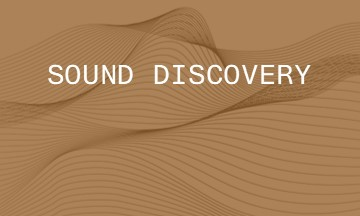
\includegraphics[width=1.0\textwidth]{SOUND_DISCOVERY_Business_Card.jpg}}



\begin{document}

\maketitle



\vspace{-0.5cm}
The papers of \cite{kardous_and_shaw_2014} and \cite{kardous_and_shaw_2016} describe the experimental design and results for unweighted and A-weighted sound level measurements for selected iOS and Android smartphones using internal microphones and external microphones, respectively.  This summary is based on these two papers.  \cite{kardous_and_shaw_2015} and \cite{faber_2017} report the results of these two studies.





\vspace{-0.5cm}
\section*{Evaluation Criteria and Methods}

\vspace{-0.3cm}
\cite{kardous_and_shaw_2014} examined 9 smartphones from the January 2013 market (4 iOS devices and 5 Android devices) with internal microphones using 10 apps.  The follow up study of \cite{kardous_and_shaw_2016} used only the original 4 iOS devices and 4 of the 10 apps from the first study with two externally calibrated microphones.

\vspace{-0.5cm}
\subsection*{Criteria}

\vspace{-0.3cm}
The iOS and Android apps were chosen based on this list of occupational noise criteria:

\begin{enumerate}[itemsep=-0.2cm]
  \item Report unweighted (C/Z/flat) and A-weighted sound levels.
  \item 3 dB or 5 dB exchange rate (dosimeter level changes for exposure time changes).
  \item Slow or fast response.
  \item Equivalent continuous average sound level (Leq) or time-weight average.
  \item Build-in microphone calibration adjustment using profiles.
  \item Reporting and sharing features.
\end{enumerate}

14 apps (10 iOS and 4 Android) were examined in \cite{kardous_and_shaw_2014}.  Only the original 4 iOS apps were examined in \cite{kardous_and_shaw_2016}.






\vspace{-0.5cm}
\subsection*{Methods}

\vspace{-0.3cm}
Randomized measurements were done using a split-split plot experimental design (experimental units:  noise level - whole plot unit;  device type - split-plot unit;  app - split-split plot unit).  The statistical power analysis required 6 replication blocks to achieve a power greater than 0.924 \citep{kardous_and_shaw_2014}.  Noise level was randomized in each block, device order was randomized with each noise level, and app order was randomized in each device.  Differences in both unweighted (flat) and A-weighted sound levels measured in each test condition and the calibration reference was used to assess accuracy.

The tests done in \cite{kardous_and_shaw_2014, kardous_and_shaw_2016} used 20 Hz to 20 kHz pink noise at 7 levels from 65 dB to 95 dB in 5 dB increments, which \textit{reflected noise exposures in a typical workplace} (circa 2016).

Controlled measurements were done in a \textit{diffuse sound field} to ensure the location (microphone direction) and size of each smartphone using an internal microphone \citep{kardous_and_shaw_2014}  or an optional external microphone \citep{kardous_and_shaw_2016} did not affect the data collection;   effectively normalizing this aspect of measurement.  \cite{kardous_and_shaw_2014} notes in-field measurement conditions (i.e., temperature, humidity, stability and use-period of device) will influence measurements.

The reference measurement microphone and meter were calibrated between measurement sessions and annually at a National Institute of Standards and Technology (NIST) laboratory.


%\cite{kardous_and_shaw_2014} - internal microphone;  3 factors
%
%10 iOS Apps -> 10 * 4 = 40 * 7 = 280 samples
%4 Android Apps -> 4 * 5 = 20 * 7 = 140 samples
%
%Whole Plot - Noise Level:  Factor 1, 7 Levels (lowest precision)
%    Split Plot - Device Type (internal microphone):  Factor 2, 9 Levels
%        Split-split Plot - App:  Factor 3, 14 Levels (highest precision)

% https://www.stat.purdue.edu/~zhanghao/STAT514/Lecture_Notes/LectureNotes20-Split-plot-Designs-.html
% https://www.youtube.com/watch?v=hHPdbYYdBVA





\vspace{-0.5cm}
\subsection*{Conclusions}

\vspace{-0.3cm}
iOS devices and apps were found to be more accurate.  In \cite{kardous_and_shaw_2014}, the \textit{SPLnFFT} app has the best agreement in unweighted SPLs, while the \textit{SoundMeter} app had the best agreement in A-weighted SPLs.  The iPhone 3GS with its internal microphone was used in both cases.

For the iOS devices, external microphones improved the accuracy and precision of noise measurements \citep{kardous_and_shaw_2016} for all 4 of the original iOS apps (\textit{SPLnFFT}, \textit{SoundMeter}, \textit{SPL Pro}, and, \textit{NoiSee}).  \textit{It is suggested that the internal microphone is the primary reason for poor accuracy and precision, not the app or smartphone hardware.}

The advantages and disadvantages of using smartphones as sound level meters are,

\vspace{-0.5cm}
\subsubsection*{Advantages}

\vspace{-0.3cm}
\begin{itemize}[itemsep=-0.15cm]
    \item Sound level apps are readily and widely available and do not require specialized knowledge.
    \item Relative good accuracy and precision allowing for good initial measurements and evaluation.
    \item Improve awareness of workplace noise and advocate for the hearing health of workers.
    \item Improved accuracy by using an external microphone.  Calibration profiles for external microphones are provided by some app developers.
\end{itemize}

\vspace{-0.6cm}
\subsubsection*{Disadvantages}

\vspace{-0.3cm}
\begin{itemize}[itemsep=-0.15cm]
    \item Phone body shape will influence the microphone, particularly at high frequencies \citep{faber_2017}.
    \item The directionality of internal microphones is not known.
    \item Calibration of external microphones requires a calibrator and training.
    \item Cost of external calibrator might be prohibitive \citep{kardous_and_shaw_2016}.
    \item Potential microphone coupling problems with the external calibrator \citep{kardous_and_shaw_2016}.
    \item External microphone performance might change with time, handling, and measurement conditions.
    \item External microphones may not be factually comply with standards \citep{kardous_and_shaw_2016}.
    \item As of 2016, no smartphone-based sound level measurement solution has met all the electrical and acoustical requirements of the American National Standards Institute (ANSI;  1983) and the International Electrotechnical Commission (IEC;  2013).
\end{itemize}





\vspace{-0.5cm}
\section*{Decision}

\vspace{-0.5cm}
I have decided to purchase an XL2 sound level meter and a Class 2 microphone from NTI.  This meter and microphone system has calibration certification and meets the IEC 61672 and ANSI S1.4 standards.





%\section*{Secondary Comments}
%
%\vspace{-0.25cm}
%I found the disclosure of the author in \cite{faber_2017} interesting, only as a footnote and an indirect statement in his biography.  I would have thought a standard disclosure statement would have been required by the editors of Acoustics Today given his involvement with sound measurement app development with Faber Acoustical, LLC.





\vspace{-0.5cm}
\bibliography{ACS_537_Project_1_Bibliography}

%\begin{thebibliography}{9}  % 9 characterizes the alignment of the indices.
%
%\bibitem{faber_2017}
%B. M. Faber (2017), \emph{Acoustical Measurements with Smartphones:  Possibilities and Limitations},
%Acoustics Today, Summer 2017, Volume 13, Issue 2, pages 10 to 17
%
%\bibitem{kardous_and_shaw_2014}
%C. A. Kardous, P. B. Shaw (2014), \emph{Evaluation of smartphone sound measurement applications},
%Journal of the Acoustical Society of America, Express Letters, Volume 135, Issue 4, pages EL186 to EL192
%
%\bibitem{kardous_and_shaw_2015}
%C. A. Kardous, P. B. Shaw (2015), \emph{Do Sound Meter Apps Measure Noise Levels Accurately?},
%Sound and Vibration, July, pages 10 to 13
%
%\bibitem{kardous_and_shaw_2016}
%C. A. Kardous, P. B. Shaw (2016), \emph{Evaluation of smartphone sound measurement applications (apps) using external microhones - A follow-up study},
%Journal of the Acoustical Society of America, Express Letters, Volume 140, Issue 4, pages EL327 to EL333
%
%
%%% Additional papers:
%
%%   https://www.sciencedirect.com/science/article/abs/pii/S0003682X17309945
%
%%   https://www.ncbi.nlm.nih.gov/pmc/articles/PMC10686533/#:~:text=The%20results%20of%20one%20simulation,(A)%20%5B6%5D.
%
%%   https://www.tandfonline.com/doi/full/10.1080/15459624.2016.1183014
%
%
%\end{thebibliography}


\end{document}




